Consider the first example.

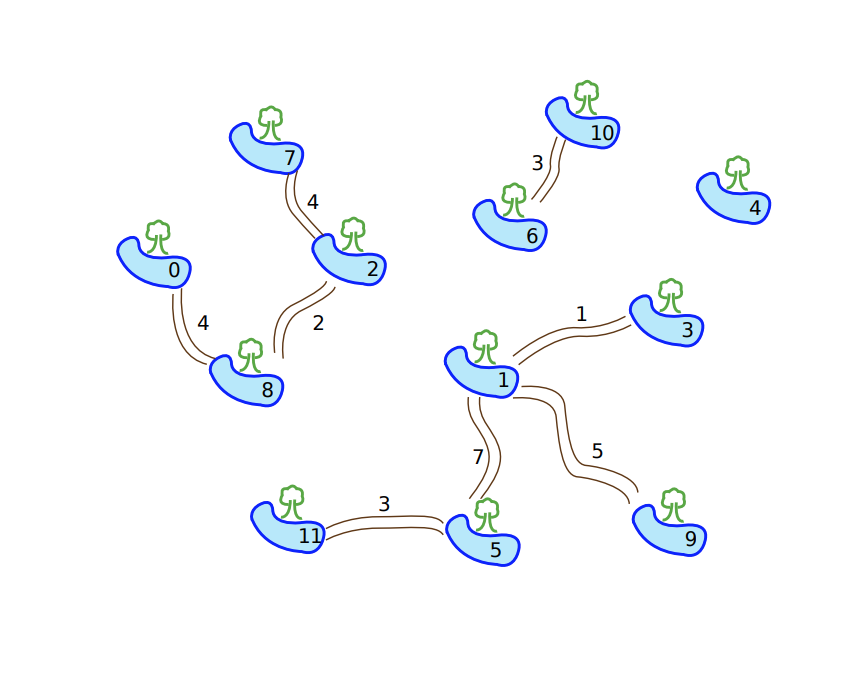
\includegraphics{dreaming1.png}

In the picture above there are $N = 12$ billabongs and $M = 8$ trails. Suppose that $L = 2$ , so that any new trail will require Serpent $2$ days to travel. Then Kangaroo could build three
new trails:
\begin{itemize}
\item between billabongs $1$ and $2$;
\item between billabongs $1$ and $6$;
\item between billabongs $4$ and $10$.
\end{itemize}

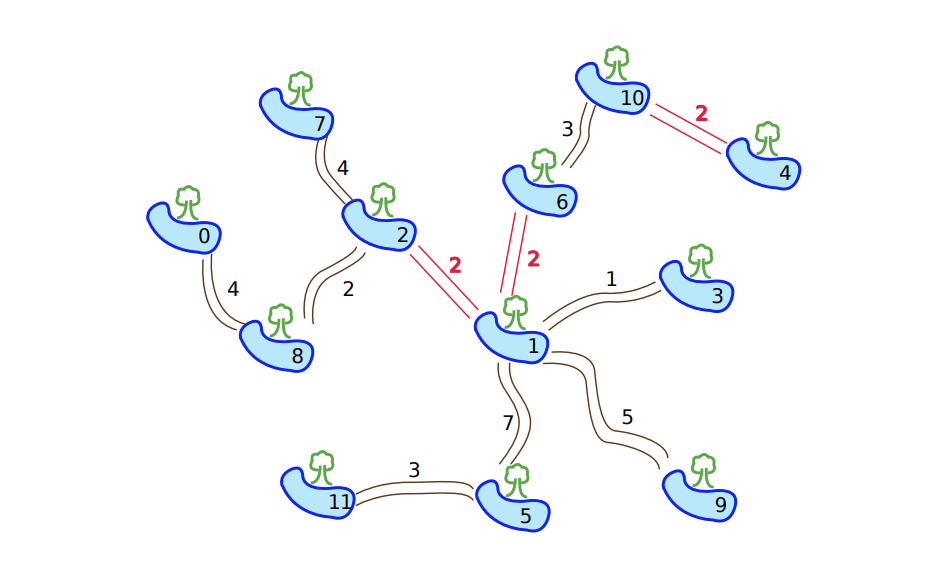
\includegraphics{dreaming2.png}

The picture above shows the final set of trails. The longest travel time is $18$ days, between
billabongs $0$ and $11$. This is the smallest result possible---no matter how Kangaroo builds
the trails, there will be some pair of billabongs that requires Serpent to travel for $18$ days or
more.

Your submission should \t{\#include ``dreaming.h"}.